\documentclass[a4paper]{article}

%% Language and font encodings
\usepackage[english]{babel}
\usepackage[utf8x]{inputenc}
\usepackage[T1]{fontenc}

%% Sets page size and margins
\usepackage[a4paper,top=3cm,bottom=2cm,left=3cm,right=3cm,marginparwidth=1.75cm]{geometry}

%% Useful packages
\usepackage{amsmath}
\usepackage{mathtools}
\usepackage{graphicx}
\usepackage{bigstrut}
\usepackage{numprint}
\usepackage{color}
\usepackage{float}
\usepackage[figurename=Figura]{caption}
\usepackage[tablename=Tabella]{caption}

\makeatletter
\def\BState{\State\hskip-\ALG@thistlm}
\makeatother

\title{\textbf{Insertion Sort e Radix Sort}}
\author{Lorenzo Pesci}
\date{6 Luglio 2020}

\begin{document}
\maketitle

\section{Introduzione}
Vogliamo analizzare le differenze fra gli algoritmi di Insertion Sort e Radix Sort per ordinare un numero crescente di valori.
\newline
Entrambi gli algoritmi sono algoritmi di ordinamento, che ricevono in input una sequenza di numeri casuali e restituiscono in output una sequenza di numeri ordinati.

\subsection{Insertion Sort}
Insertion Sort \'e l'algoritmo pi\'u semplice per il risolvere il problema dell'ordinamento, e risulta efficiente per input di piccole dimensioni.
\newline
Riceve in input un array A, i cui numeri sono ordinati sul posto: ossia in ogni istante ci sono al pi\'u un numero costante di valori memorizzati all'esterno di A.
\newline
\newline
\textbf{Pseudocodice:}
\newline
\newline
INSERTION-SORT (A)
\newline
1 for j = 2 to length[A]
\newline
2 \hspace{18pt} key = A[j]
\newline
3 \hspace{18pt} i = j - 1
\newline
4 \hspace{18pt} while i > 0 and A[i] > key
\newline
5 \hspace{45pt} A[i + 1] = A[i]
\newline
6 \hspace{47pt} i = i - 1
\newline
7 \hspace{18pt} A[i + 1] = key
\newline
\newline
Nel nostro esperimento, lo pseudocodice proposto viene tradotto in linguaggio Python nel file insertionsort.py

\subsection{Radix Sort}
Radix Sort \'e un algoritmo che riceve in input un array A in cui ogni valore \'e composto di d cifre. Inizialmente ordina A usando la cifra meno significativa di ogni numero come chiave di ordinamento, poi ripete l'ordinamento utilizzando come chiave la seconda cifra significativa e cos\'i via, finch\'e non saranno state considerate tutte le d cifre. 
\newline
Radix Sort si avvale di un algoritmo di ordinamento ausiliario, e fondamentale per la sua correttezza \'e che questo algoritmo ausiliario sia stabile, quindi Counting Sort \'e un ottimo candidato.
\newline
\newline
\textbf{Pseudocodice:}
\newline
\newline
RADIX-SORT(A,d)
\newline
1 for i = 1 to d
\newline
2 \hspace{18pt} usa un ordinamento stabile per ordinare A usando come chiave la cifra i
\newline
\newline
Nello pseudocodice di Radix Sort si suppone che la cifra 1 sia la meno significativa e la cifra d la pi\'u significativa.
\newline
Nel nostro esperimento, lo pseudocodice proposto viene tradotto in linguaggio Python nel file radixsort.py

\section{Descrizione esperimenti e documentazione del codice}
Gli esperimenti sono stati svolti su un MacBook Pro con sistema operativo macOS Catalina, processore 2,2 GHz 6-Core Intel Core i7 e 16 GB di RAM.
\newline
\newline
Eventuali numeri casuali sono stati generati dalla funzione \textit{random.randint()} importata dalla libreria \textit{random}.
\newline
\newline
Il codice è articolato in quattro file: $insertionsort.py$, $radixsort.py$, $plot.py$, $main.py$.
\newline
\newline
- Nel file \textbf{insertionsort.py} \'e realizzato in linguaggio Python l'algoritmo di Insertion Sort che verr\'a utilizzato per i nostri esperimenti.
\newline
\newline
- Nel file \textbf{radixsort.py} \'e realizzato in linguaggio Python l'algoritmo di Radix Sort che verr\'a utilizzato per i nostri esperimenti.
\newline
\newline
- Nel file \textbf{plot.py} sono realizzati tutti i grafici sugli esperimenti condotti sia su Insertion Sort che su Radix Sort.
\newline
\newline
- Nel  file \textbf{main.py} \'e realizzato il codice che esegue i test su entrambi gli algoritmi. In particolare sono stati eseguiti dei test diversi per entrambi gli algoritmi riguardanti in problema dell'ordinamento. 
\newline
\clearpage
\section{Presentazione dati sperimentali}

\subsection{Insertion Sort}

Sull'algoritmo di Insertion Sort sono stati eseguiti i test su un numero crescente di elementi, partendo da array di cento elementi fino a raggiungere un array con centomila elementi, analizzando il tempo di esecuzione dell'algoritmo. 
\newline
In particolare sono stati realizzati tre esperimenti considerando il caso migliore, il caso peggiore e il caso medio di Insertion Sort, ovvero rispettivamente ordinamento su array ordinato, array ordinato al contrario e array generato randomicamente.
\newline
\newline
Di seguito \'e riportata la \textbf{tabella} del tempo di esecuzione di Insertion Sort sui tre casi.

\begin{center}
\begin{table}[h!]
\centering
\begin{tabular}{|l|l|l|l|l|}

\hline
\textbf{Numero di Elementi} & \textbf{100} & \textbf{1000} & \textbf{10000} & \textbf{100000}\\
\hline
\textbf{Array Random} & 0.00027 & 0.02481 & 2.01623 & 199.041\\
\hline
\textbf{Array Ordinato} & 1.5020e-05 & 0.00010 & 0.00103 & 0.01214   \\
\hline
\textbf{Array Ordinato Al Contrario} & 0.00040 & 0.03872 & 3.82862 & 409.713  \\
\hline
\end{tabular}
\caption{Tabella tempo di esecuzione di Insertion Sort}
\end{table}
\end{center}

Come si evince dai risultati ottenuti l'algoritmo ed i test implementai rispettano la teoria, ovvero il caso migliore si ha con array ordinato, il caso medio si ha con array generato randomicamente ed infine il caso peggiore si ha con array ordinato al contrario.

Di seguito sono riportati i \textbf{grafici} di Insertion Sort per ognuno dei tre casi analizzati.

\begin{figure}[h]
    \centering
    \captionsetup{justification=centering,margin=1.0cm}
    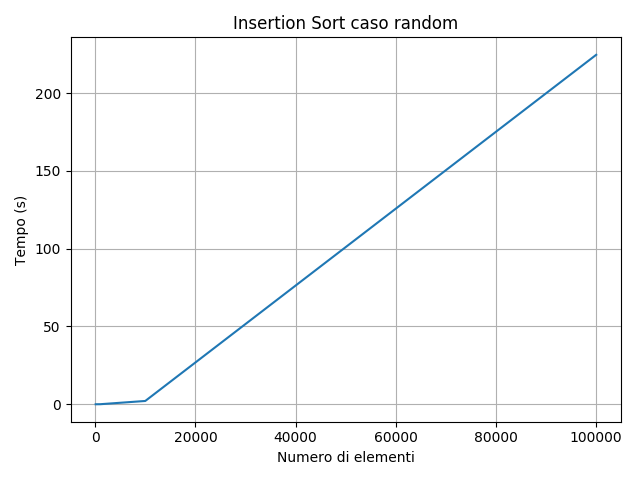
\includegraphics[width=0.7\textwidth]{IS_random}
    \caption{Tempo di esecuzione di Insertion Sort su array random.}
    \label{fig:test2_1}
\end{figure}


\begin{figure}[h]
    \centering
    \captionsetup{justification=centering,margin=1.0cm}
    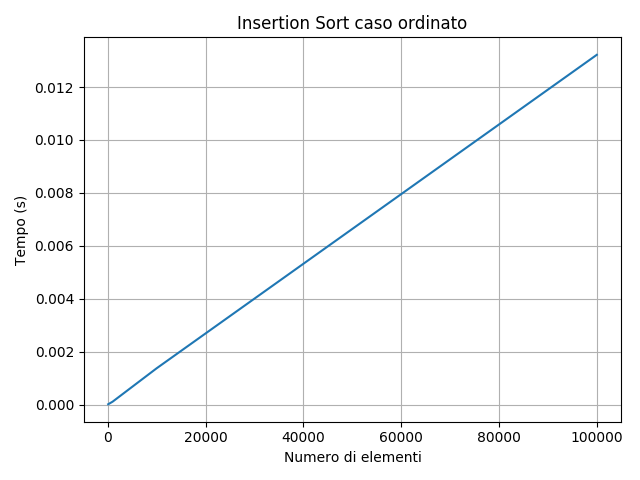
\includegraphics[width=0.7\textwidth]{IS_ordinato}
    \caption{Tempo di esecuzione di Insertion Sort su array ordinato.}
    \label{fig:test2_1}
\end{figure}

\begin{figure}[h]
    \centering
    \captionsetup{justification=centering,margin=1.0cm}
    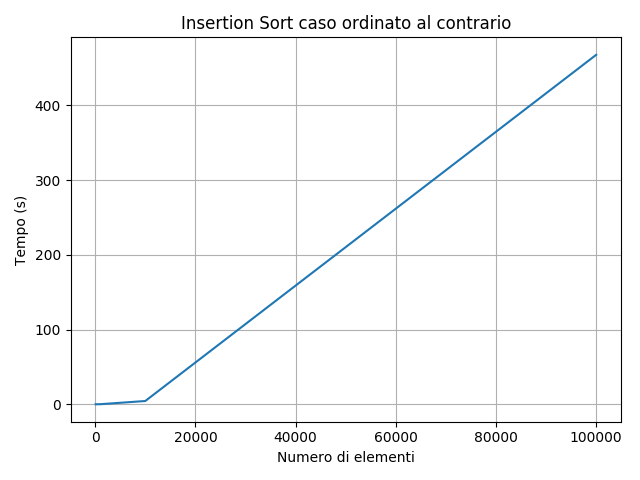
\includegraphics[width=0.7\textwidth]{IS_ordincontr}
    \caption{Tempo di esecuzione di Insertion Sort su array ordinato al contrario.}
    \label{fig:test2_1}
\end{figure}
\clearpage

\subsection{Radix Sort}
Per l'algoritmo di Radix Sort sono stati condotti due tipi di esperimenti.
\newline
\subsubsection{Primo esperimento}
Il primo esperimento \'e stato condotto variando la base con cui viene rappresentato un numero. In particolare sono state utilzzate la base 2, la base 5 e la base 10, ovvero la base decimale con la quale abbiamo a che fare ogni giorno nella vita quotidiana. Oltre alla base del numero, l'esperimento tiene conto di un numero crescente di elementi, ovvero siamo partiti da cento elementi in base 2, base 5 e base 10 fino ad arrivare a centomila elementi in base 2, base 5 e base 10. 
\newline
Di seguito \'e riportata la \textbf{tabella} riassuntiva dei risultati ed il \textbf{grafico} di confronto dei risultati.

\begin{center}
\begin{table}[h!]
\centering
\begin{tabular}{|l|l|l|l|l|}
\hline
\textbf{Numero di Elementi} & \textbf{100} & \textbf{1000} & \textbf{10000} & \textbf{100000}\\
\hline
\textbf{Base 2} & 0.00135 & 0.01310 & 0.14778 & 1.46151\\
\hline
\textbf{Base 5} & 0.00042 & 0.00403 & 0.04126 & 0.39812\\
\hline
\textbf{Base 10} & 0.00029 & 0.00323 & 0.03747 & 0.33712\\
\hline
\end{tabular}
\caption{Tabella tempo di esecuzione di Radix Sort}
\end{table}
\end{center}


\begin{figure}[h]
    \centering
    \captionsetup{justification=centering,margin=1.0cm}
    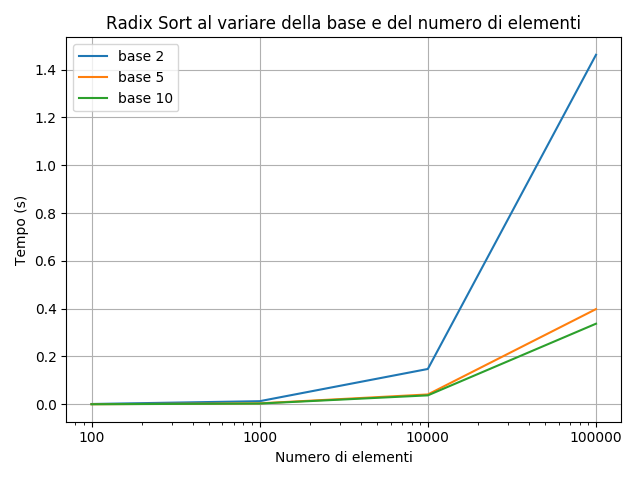
\includegraphics[width=0.7\textwidth]{RS_Basi}
    \caption{Tempo di esecuzione di Radix Sort in base 2, base 5 e base 10.}
    \label{fig:test2_1}
\end{figure}

Come ci aspettavamo dai dati teorici, Radix Sort risulta pi\'u efficente sui numeri in base 10, poich\'e ordina numeri su pi\'u cifre significative ma su un numero inferiore di bit.

\subsubsection{Secondo esperimento}
Per la seconda parte dell'esperimento abbiamo quindi utlizzato la base 10 come notazione per rappresentare i nostri numeri. In questo esperimento abbiamo utlizzato array che partivano da cento elementi fino ad arrivare ad un milione di elementi variando il numero massimo da ordinare. 
\newline
Di seguito \'e riportata la \textbf{tabella} riassuntiva dei risultati ed il \textbf{grafico} di confronto dei risultati.
\clearpage

\begin{center}
\begin{table}[h!]
\centering
\begin{tabular}{|l|l|l|l|l|}

\hline
\textbf{Numero di Elementi} & \textbf{100} & \textbf{1000} & \textbf{10000} & \textbf{100000}\\
\hline
\textbf{Da 1 a 100} & 0.00030 & 0.00370 & 0.03335 & 0.33719\\
\hline
\textbf{Da 1 a 1000} & 0.00038 & 0.00451 & 0.06099 & 0.42153\\
\hline
\textbf{Da 1 a 10000} & 0.00045 & 0.00486 & 0.07889 & 0.52280\\
\hline
\textbf{Da 1 a 100000} & 0.00053 & 0.00535 & 0.06909 & 0.63612\\
\hline
\textbf{Da 1 a 1000000} & 0.00061 & 0.00671 & 0.08480 & 0.68152\\
\hline
\end{tabular}
\caption{Tabella tempo di esecuzione di Radix Sort al variare del numero massimo da ordinare e del numero di elementi.}
\end{table}
\end{center}

\begin{figure}[h]
    \centering
    \captionsetup{justification=centering,margin=1.0cm}
    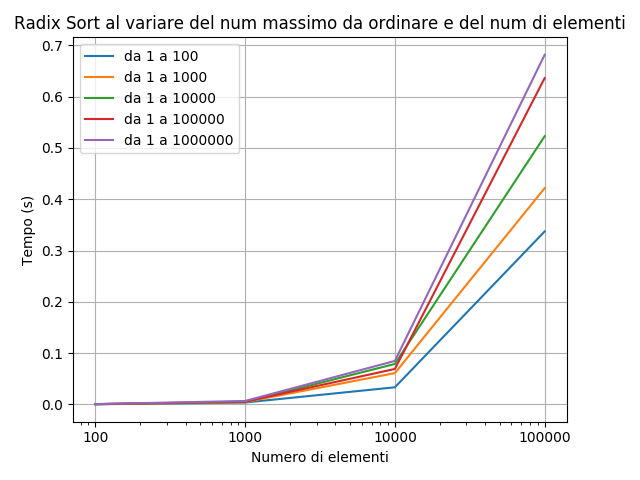
\includegraphics[width=0.7\textwidth]{RS_NumMax_NumElem}
    \caption{Radix Sort al variare del numero massimo da ordinare e del numero di elementi.}
    \label{fig:test2_1}
\end{figure}

Infine, come nel caso di Insertion Sort, sono stati condotti gli esperimenti inserendo in input la stessa sequenza di array nel caso in cui l'array fosse ordinato o ordinato al contrario.

\begin{center}
\begin{table}[h!]
\centering
\begin{tabular}{|l|l|l|l|l|}
\hline
\textbf{Numero di Elementi} & \textbf{100} & \textbf{1000} & \textbf{10000} & \textbf{100000}\\
\hline
\textbf{Array Ordinato} & 8.296e-05 & 0.00105 & 0.01455 & 0.21112\\
\hline
\textbf{Array Ordinato Al Contrario} & 5.960e-06 & 2.002e-05 & 0.00018 & 0.00181 \\
\hline
\end{tabular}
\caption{Tabella tempo di esecuzione di Radix Sort su array ordinato e array ordinato al contrario}
\end{table}
\end{center}

\begin{figure}[h]
    \centering
    \captionsetup{justification=centering,margin=1.0cm}
    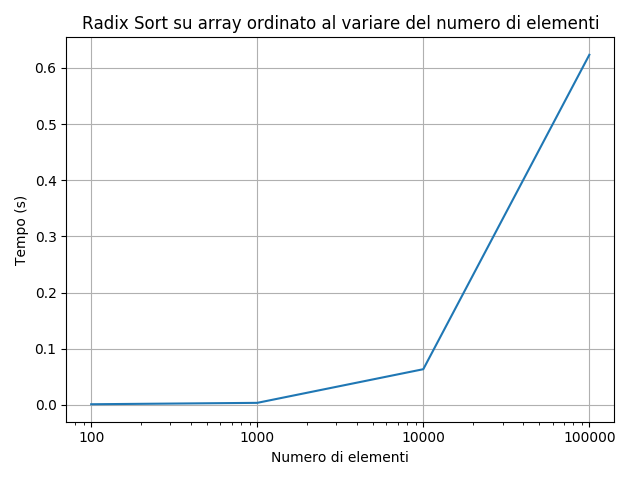
\includegraphics[width=0.7\textwidth]{RS_Ordinato}
    \caption{Tempo di esecuzione di Radix Sort su array ordinato.}
    \label{fig:test2_1}
\end{figure}

\begin{figure}[h]
    \centering
    \captionsetup{justification=centering,margin=1.0cm}
    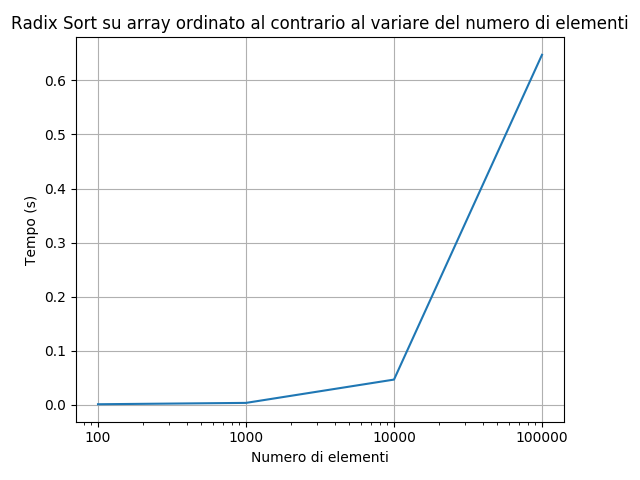
\includegraphics[width=0.7\textwidth]{RS_Ordinato_Contrario}
    \caption{Tempo di esecuzione di Radix Sort su array ordinato al contrario}
    \label{fig:test2_1}
\end{figure}

\clearpage

\section{Analisi dei risultati ottenuti}

Dai nostri test possiamo vedere come il caso di Array Ordinato con Insertion Sort è quello che impiega il minor tempo di esecuzione.
Tale risultato si poteva intuire anche dalla teoria, avendo un costo computazionale pari a $\theta$($n$).
\newline
Negli altri casi invece Radix Sort è generalmente più veloce e tale rapidità rimane costante in tutti i casi, questo è dovuto alla
sua complessità totale pari a $\theta$($n$).
\newline
Una grande diversità tra i tempi di esecuzione si può notare nel caso di Array Random e Array Ordinato al Contrario con 100000 elementi, dove il Radix Sort esegue l'ordinamento in poco più di un decimo di secondo, invece l'Insertion Sort impiega qualche minuto per portare a termine l'operazione.
\newline
Quindi generalmente, avendo un tempo totale di esecuzione $\theta$($n$), il Radix Sort è un algoritmo che impiega con i nostri dati sempre meno di un secondo per completare l'ordinamento.
\newline
Con tali esperimenti possiamo dunque comprendere quanto sia grande la differenza tra avere un costo computazionale
pari a $\theta$($n$) o $\theta$($n^2$).
\newline

\section{Conclusioni}
Anche se Radix Sort e Counting Sort vengono eseguiti in un tempo asintoticamente lineare, algoritmi di ordinamento sul posto vengono comunque preferiti a questi due algoritmi.
\newline
Infatti quest'ultimi eseguono l'ordinamento sul posto senza utilizzare un array ausiliario o produrre un nuovo array per il risultato. Infine i fattori costanti nascosti nella notazione $\theta$($n$) possono produrre un tempo di esecuzione superiore rispetto a un ordinamento per confronti.

\begin{center}
\begin{table}[h!]
\centering
\begin{tabular}{|l|l|l|l}
\hline
\textbf{TEMPO DI ESECUZIONE} & \textbf{INSERTION SORT} & \textbf{RADIX SORT}\\
\hline
\textbf{Array Random} & $\theta$($n^2$) & $\theta$($n$)\\
\hline
\textbf{Array Ordinato} & $\theta$($n$) & $\theta$($n$)\\
\hline
\textbf{Array Ordinato Al Contrario} & $\theta$($n^2$) & $\theta$($n$) \\
\hline
\end{tabular}
\caption{Tabella dei Costi}
\end{table}
\end{center}


\end{document}
